\section{Grundlagen der Datenanalyse}\label{chap:GrundlagenDatenanalyse}

Mathematisch ausgedrückt besteht eine Zeitreihe (im englischen auch \enquote{time series} genannt) aus einer endlichen Menge an zeitlich aufsteigend sortierten Messwerten $x_{t_1},x_{t_2},...,x_{t_T};  x_{t_k} \in \mathbb{R}^n, k=1,2,...,T$, wofür $t_1 < t_2 < t_T $ gilt.\footcite[Vgl.][1]{Deistler.2018b} 
Zeitreihendaten sind in verschiedenen Feldern zu finden, beispielsweise im Bereich der Aktienmärkte, wo die Preise der einzelnen Kurse abgebildet werden, im Bereich der Gesundheitsforschung, wo die Ansteckungsrate ansteckender Krankheiten wie Covid-19 verfolgt wird oder im Bereich der Sozialwissenschaften, in welchen der Verlauf von Geburtsraten über die Zeit analysiert werden soll.\footcite[Vgl.][1]{Shumway.2017b} 
In \autoref{abb:BeispielZeitreihe} findet sich beispielhaft die Zeitreihe der zwei messbaren Feinstaubkategorien von null bis ein Uhr am 01.01.2020 in Stuttgart.

\begin{figure}[H]
\centering
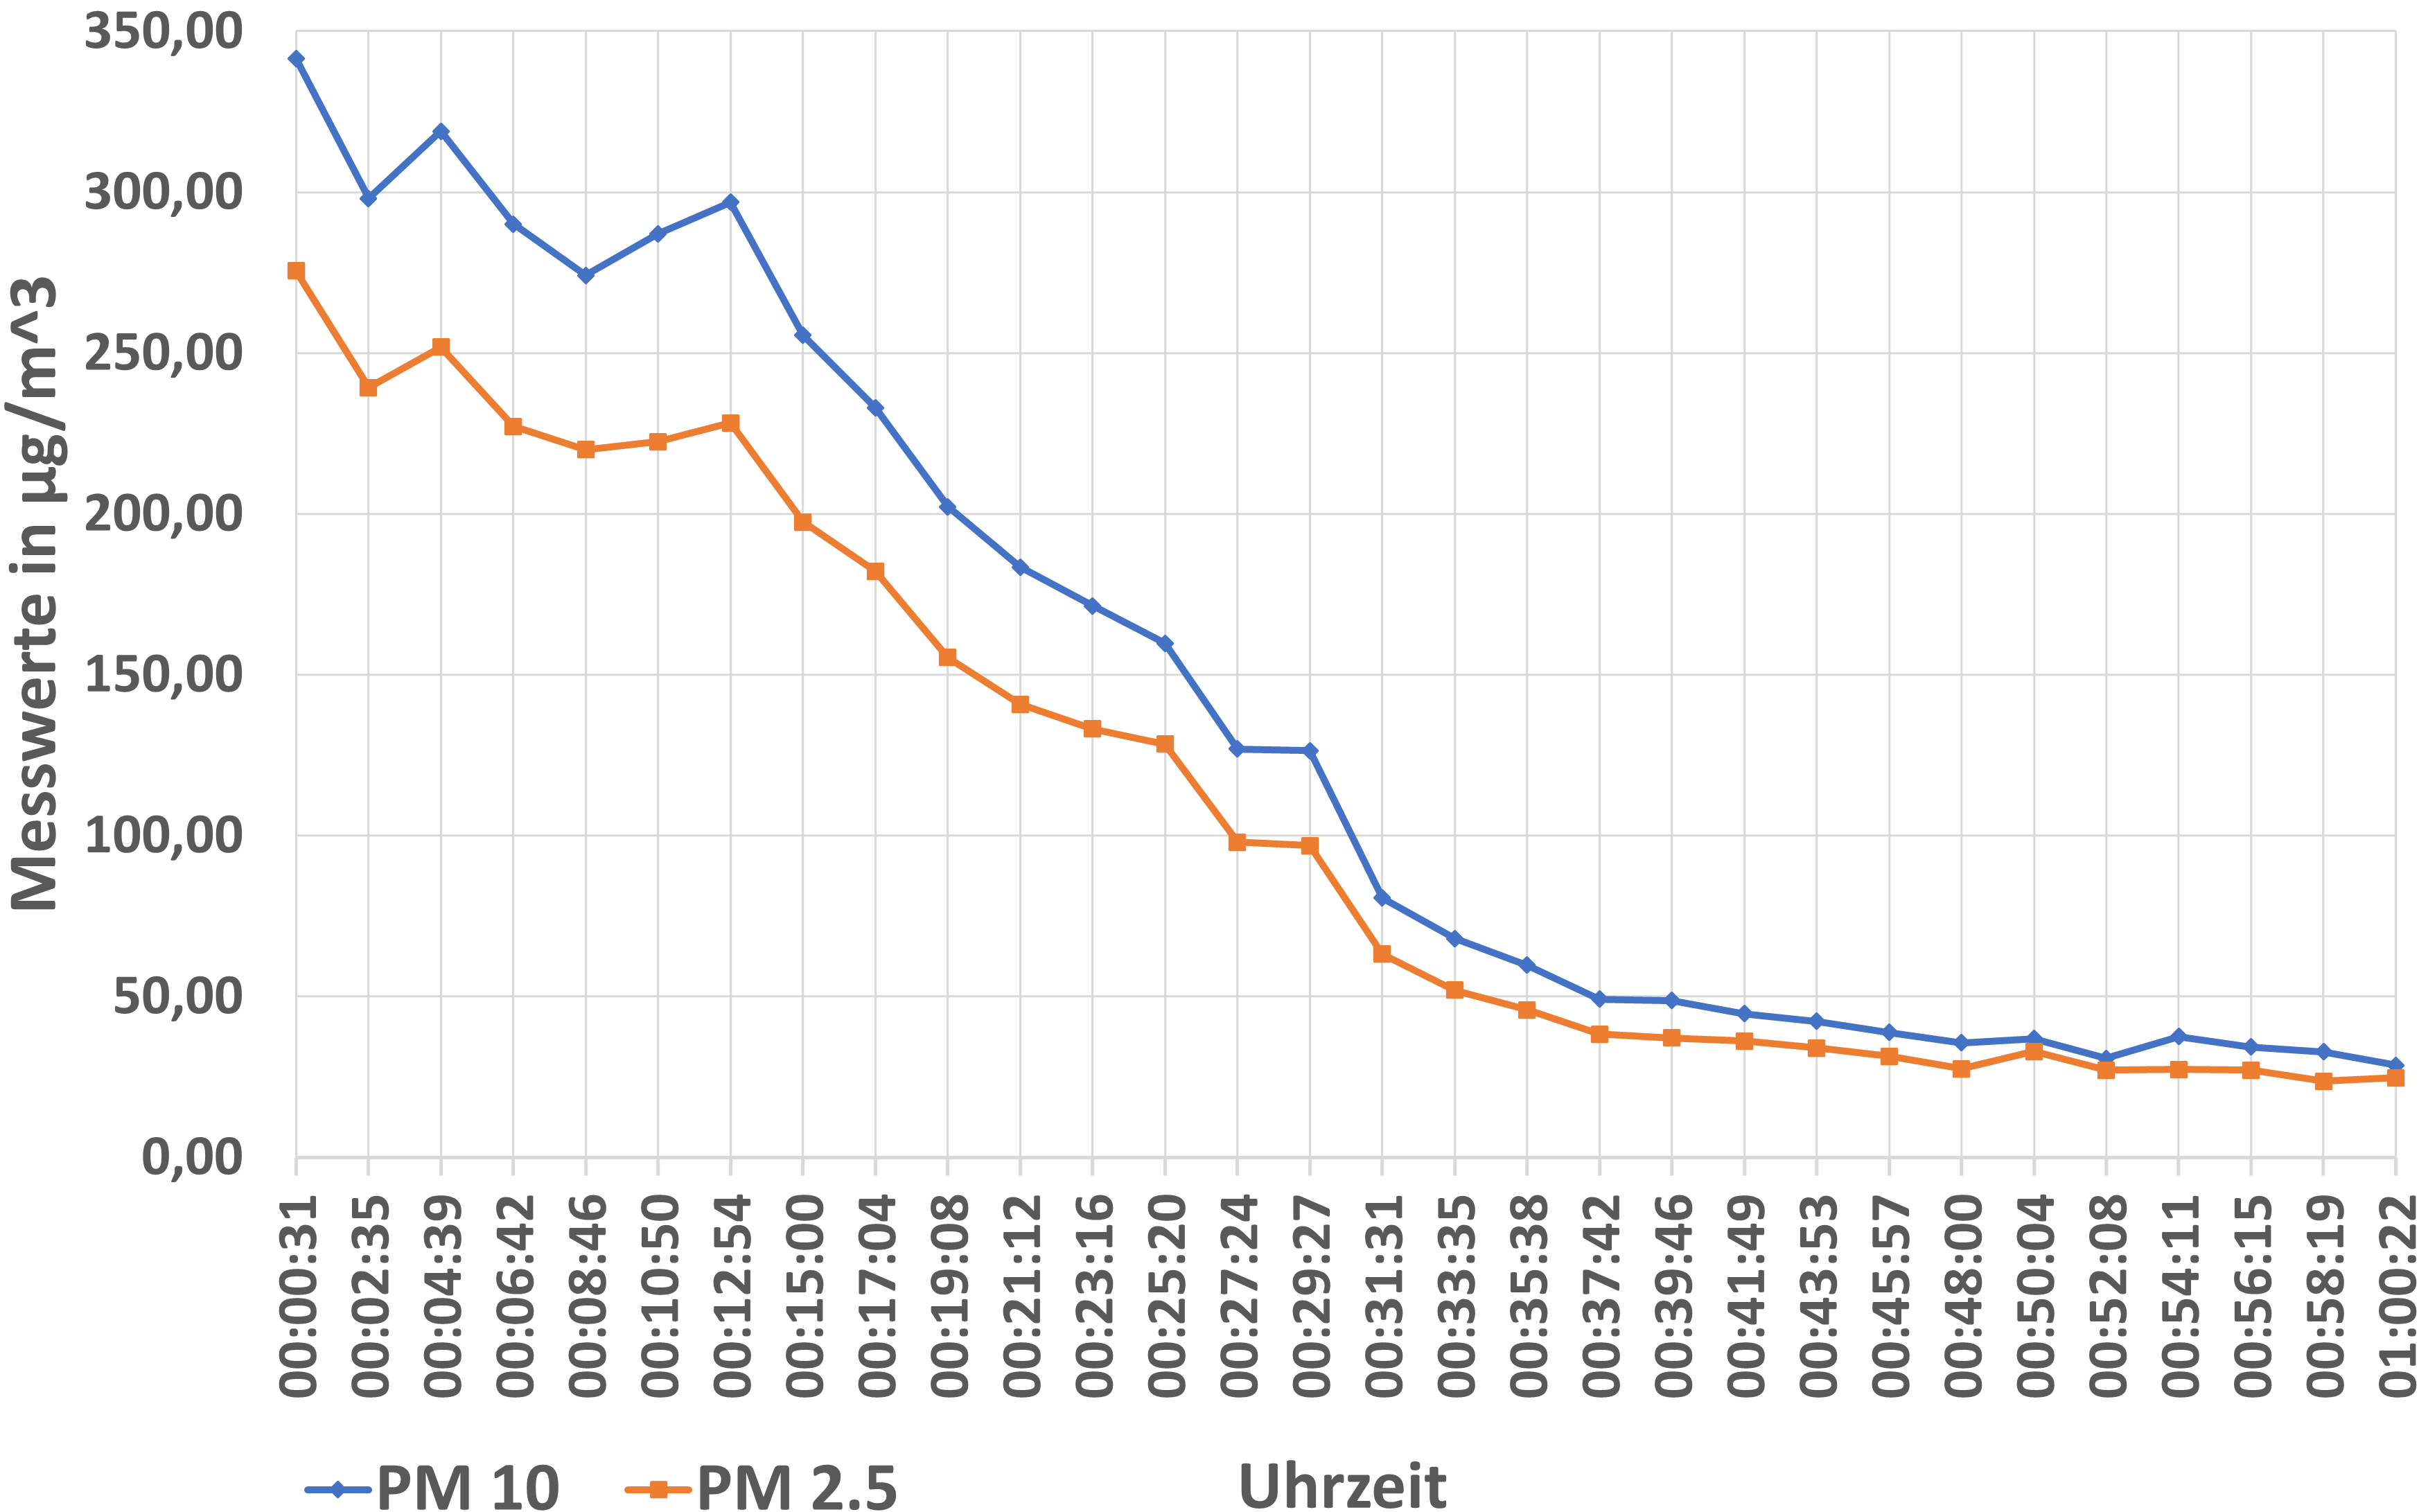
\includegraphics[width=\textwidth]{graphics/Feinstaub-Stuttgart.png}
\caption{Beispielhafte Zeitreihe von der Stunde nach Jahreswechsel 2020}
\label{abb:BeispielZeitreihe}
\end{figure}

Die möglichen Anwendungen in der Informatik sind ebenfalls vielzählig. So können über virtuelle oder physikalische Sensoren Messwerte, wie beispielsweise die CPU Auslastung eines gegebenen Servers über die Zeit oder Temperaturmessungen eines \ac{IoT} Gerätes über die Zeit gemacht und gespeichert werden.

Ein wichtiges Merkmal von Zeitreihen ist die Distanz zwischen den Messwerten, im Sinne der Messfrequenz, in welcher Daten betrachtet werden. \Todo{belegen} Ist eine Zeitreihe äquidistant, wurde mit gleichbleibender Frequenz gemessen und die zeitliche Distanz zwischen einzelnen Messwerten ist gleich. Für die in dieser Arbeit diskutierten Auswertungsarten wird eine Äquidistanz der gemessenen Daten angenommen, da andernfalls ein Bias/eine Verfälschung bei der Analyse nicht ausgeschlossen werden kann. Gleichfalls ist es technisch möglich einzelne, nicht äquidistante Messwerte auszusortieren oder fehlende Messwerte zu interpolieren. Die in \autoref{abb:BeispielZeitreihe} abgebildete Zeitreihe ist äquidistant, da die Werte alle 124 Sekunden erhoben wurden.

Es ist von zwei vorliegenden Typen von Zeitreihendaten auszugehen. Zum einen existiert der mit Zeitstempel versehene Messwert, welcher einen oder in manchen Fällen auch mehrere diskrete Messwerte mit Zeitstempel der Erfassung übermittelt. 
Zum anderen existieren auch Ereignisse, welche keine Messwerte enthalten, sondern Ergebnisse einer Vorauswertung innerhalb des übermittelnden Systems sind. 
So wäre ein Ereignis beispielsweise ein niedriger Batteriestand eines verbundenen Sensors. 
Abhängig von der Vorauswertung werden Ereignisse einmal, nach Auftreten mit Zeitstempel oder periodisch mit Zeitstempel bis zum Beheben der Ursache versendet. \Todo{belegen}

\subsection{Analysewert verarbeiteter Daten}

Bei der Verarbeitung von Daten ist zu beachten, dass der Wert, bzw. die Erkentnisse die aus den Daten abgleitet werden können, über die Zeit reduziert wird. \footcite[Vgl. auch im Folgenden][]{NucleusResarchInc..2012} Gemäß \citeauthor{NucleusResarchInc..2012} haben dabei verschiedene Unternehmen verschiedene Zeiträume, in denen Daten nützlich sind, da sie sich in eine von drei Entscheidungstempi einkategorisieren lassen.\footcite[Vgl. auch im Folgenden][3]{NucleusResarchInc..2012} Die \hyphenation{Entscheidungstempi} sind taktisch, operativ und strategisch. Beim taktischen Entscheidungstempo werden Änderungen sehr schnell, nahe Echtzeit getroffen und implementiert. Im Gegensatz dazu werden Entscheidungen der operativen und strategischen \hyphenation{Entscheidungstempi} respektive erst in Tagen bzw. Wochen oder innerhalb einem Quartal oder länger implementiert. Je nach Entscheidungstempo sind Analysen von eingehenden Daten also wesentlich früher notwendig oder können beispielsweise auch nur einmal täglich erstellt werden.

% \footcite[Vgl. auch im Folgenden][3]{NucleusResarchInc..2012}
% The value of data diminishes based on the cadence of decisions. Decision tempos are
% tactical (driving process changes in near real time), operational (driving changes that take
% days or weeks to implement), or strategic (driving changes that become part of a quarterly
% or longer planning and implementation process). The concept of half life, with diminishing
% value curves based on a company’s decision tempo, can be used to help companies
% measure the impact of prioritizing their data management and analytics investments. 



Für Unternehmen mit taktischem Entscheidendungstempo haben, gemäß der in \autoref{abb:DataHalflife} gezeigten Befragungsergebnisse von \citeauthor{NucleusResarchInc..2012}, Daten nach maximal 30 Minuten die Hälfte des Wertes eingebüßt.\footcite[Vgl. auch im Folgenden][6]{NucleusResarchInc..2012} Für operative \hyphenation{Entscheidungstempi} ist die durchschnittliche Halbwertszeit nach acht Stunden erreicht, für strategische \hyphenation{Entscheidungstempi} nach ca. 56 Stunden, also nach über 2 Tagen.



\begin{figure}[H]
\centering
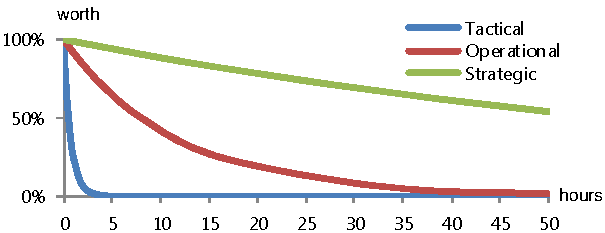
\includegraphics[width=\textwidth]{graphics/half-life-data.pdf}
\caption[Die Halbwertszeit von Daten]{Die Halbwertszeit von Daten\footnotemark}
\label{abb:DataHalflife}
\end{figure}
\footnotetext{Mit Änderungen entnommen aus: \cite{NucleusResarchInc..2012}}
Aus diesen abweichenden Halbwertszeiten und damit aus den abweichenden Zeiträumen, in denen die erhobenen Daten den höchsten Wert haben, ergibt sich die Notwendigkeit von verschiedenen Datenverarbeitungsstrategien, um entsprechend taktischen, operativen oder strategischen  Entscheidenden die werthaltigsten Daten als Entscheidungsgrundlage zu präsentieren.

\subsection{Arten der Auswertung}\label{chap:auswertungsarten}
Diese Arbeit soll anhand einiger weniger Auswertungen demonstrieren, wozu die jeweilige Referenzarchitektur und die verwendeten Dienste fähig sind. Im Folgenden werden dazu einige einfachere Auswertungsmethoden für Zeitreihendaten vorgestellt. Die Zeitreihenanalyse und einsetzbare Werkzeuge werden im statistischen Sinn von weiterführenden Werken, wie von \citeauthor{Shumway.2017} behandelt. Es ist davon auszugehen, dass auch weiterführende Auswertungen wie fourieranalytischen Methoden, sofern in der jeweiligen Umgebung bereits vorhanden oder programmierbar, eingesetzt werden können.


\subsubsection{Median und Quantile}
Eine der wichtigsten statistischen Lageparameter sind die Quantile eines Datensatzes und der Median, welcher ein spezielles, 50 prozentiges Quantil ist. 
Innerhalb eines gewissen Betrachtungsfensters können für Zeitreihendaten, wie für viele andere Datensätze auch, Quantile und der Median erfasst werden. 
Das Quantil erfasst mit der jeweiligen Prozentangabe und dem zugehörigen, ermittelten Wert die Grenze an Werten, die kleiner sind. 
Bei einem 75-\%-Quantil von $2$ wären entsprechend nur 25\% der sich im Datensatz befindlichen Daten größer als $2$. 
Da ein Median das 50-\%-Quantil ist, bildet der Median entsprechend die Grenze ab, bei welcher 50\% der Werte im Datensatz kleiner und der Rest größer ist. In \autoref{abb:quantile} sind das 25, 50 und 75-\%-Quantil auf einer modifizierten Sinusfunktion gezeigt.
\begin{figure}[H]
\centering
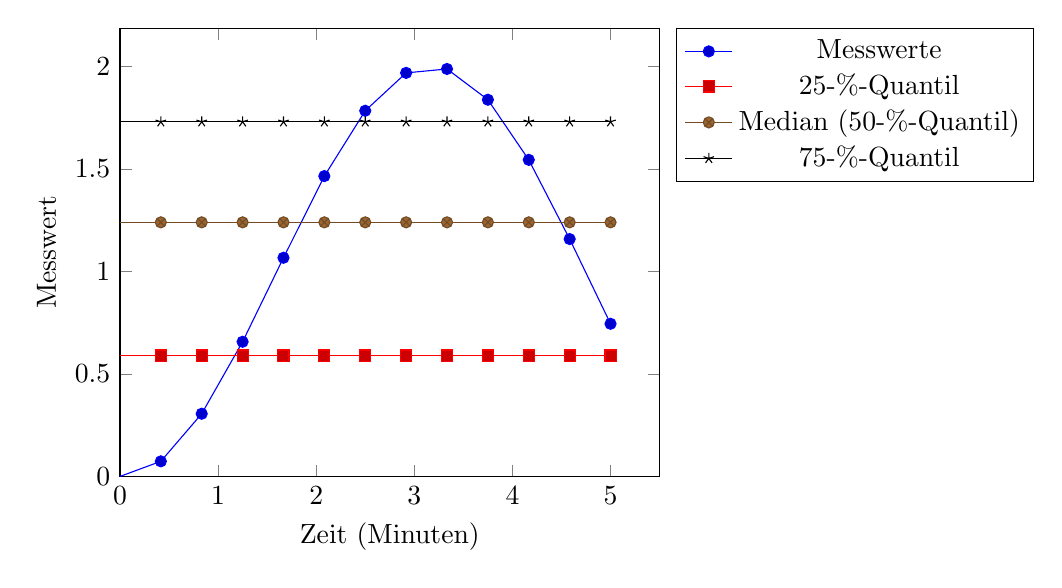
\begin{tikzpicture}
    \begin{axis}[
    xlabel=Zeit (Minuten),
    ylabel=Messwert,
    xmin=0, 
    ymin=0,
    legend pos=outer north east]
        \addplot {sin(deg(x-1.6))+1}; 
        \addplot {0.5899082};
        \addplot {1.2392493};
        \addplot {1.72939505};
        \legend{Messwerte,25-\%-Quantil,Median (50-\%-Quantil),75-\%-Quantil}
    \end{axis}
\end{tikzpicture}
\caption{Median und Quantile angewendet auf abgewandelte Sinusfunktion}
\label{abb:quantile}
\end{figure}

Gängig in der Datenanalyse als Sonderform der Quantile sind die sogenannten Perzentile, welche in einprozentigen Schritten existieren. Häufig verwendet werden insbesondere das 90-\% und das 99\% Perzentil.

\subsubsection{Anomaliedetektion}
Eine weitere gängige Datenanalysemethode ist die Anomaliedetektion. 
Dabei kann jeder Datenpunkt als Anomalie gesehen werden, der die Komplexität eines Modells, welches die Daten beschreibt, substantiell erhöhen würde.\footcite[Vgl.][]{Guha.2016} Verwandt ist dabei das Feld der \enquote{Ausreissererkennung}/outlier detection. 
Verwendet werden können dabei diverse Methodiken. Innerhalb von \ac{AWS} Produkten wird zur Anomalieerkennung ein Algorithmus basierend auf Random Cut Forest verwendet.\footcite[Vgl.][1]{Guha.2016} Weitere Methodiken wären aber auch Random Walk oder Logik basierend auf Standardannahmen.\footcite[Vgl.][]{Moonesinghe.2006}\nzitat\footcite[Vgl.][]{Angiulli.2008} Anomalien können kausal mit unterliegenden Problemen z.B. des Sensors zusammenhängen, weshalb es wichtig ist, auch abseits von den in \autoref{chap:schwellwert} gezeigten Schwellwertüberprüfungen die Daten auf Anomalien zu prüfen.

\begin{figure}[H]
\centering
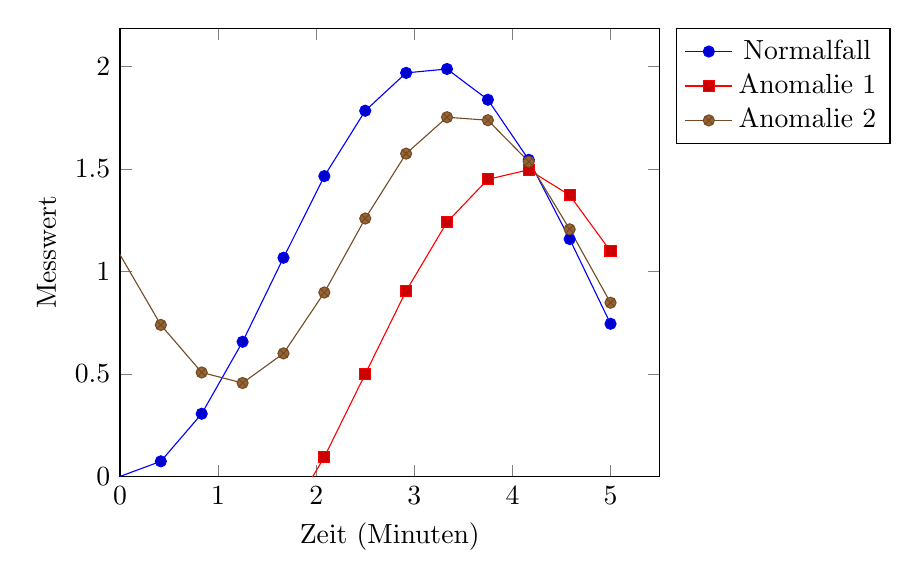
\begin{tikzpicture}
    \begin{axis}[
    xlabel=Zeit (Minuten),
    ylabel=Messwert,
    xmin=0, 
    ymin=0,
    legend pos=outer north east]
        \addplot {sin(deg(x-1.6))+1}; 
        \addplot {sin(deg(x-2.5))+0.5};
        \addplot {0.66*sin(1.33*deg(x-2.33))+1.11};
        \legend{Normalfall,Anomalie 1,Anomalie 2}
    \end{axis}
\end{tikzpicture}
\caption{Illustrierte Annomalieerkennung am Beispiel abgewandelter Sinus Funktionen}
\label{abb:anomalie}
\end{figure}

Abgebildet in \autoref{abb:anomalie} sind zwei Anomalien, die direkt in mehreren Punkten vom Normalfall abweichen.
\subsubsection{Schwellwertüberschreitung}\label{chap:schwellwert}
Bei vielen gemessenen und sonstig erfassten Zeitreihendaten, bei denen akzeptierbare Werte und Wertbereiche, die Aktionen erfordern bekannt sind, sind Schwellwerte bereits ausreichend oder komplementär verwendbar. Dabei wird, wie in \autoref{abb:Schwellwerte} gezeigt, ein Schwellwert definiert (in diesem Fall $1.75$). Zusätzlich dargestellt ist eine Karenzzeit von 12 Sekunden. Erst nach kontinuierlicher Überschreitung des Schwellwerts von 12 Sekunden wird ein Alarm ausgelöst. 
\begin{figure}[H]
\centering
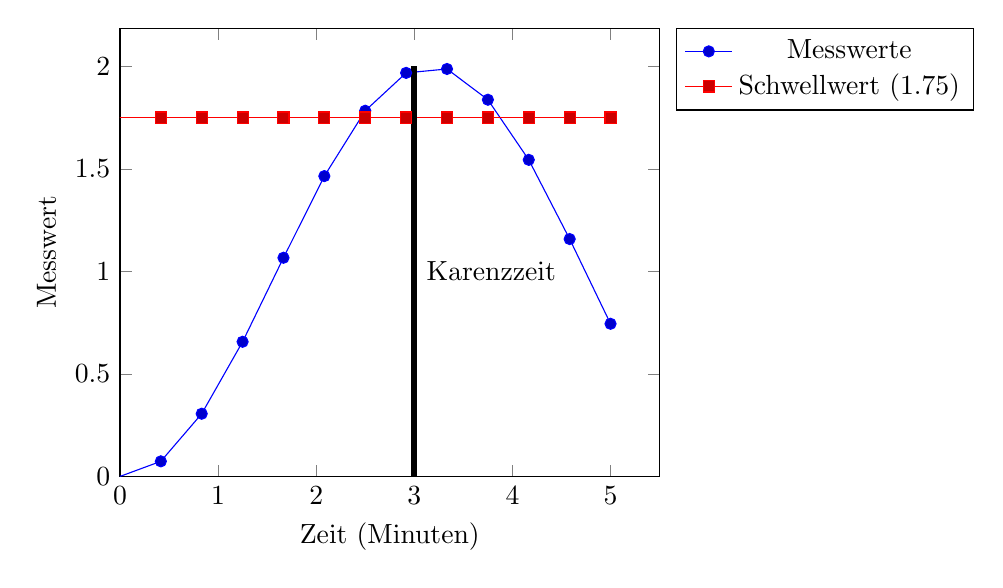
\begin{tikzpicture}
    \begin{axis}[
    xlabel=Zeit (Minuten),
    ylabel=Messwert,
    xmin=0, 
    ymin=0,
    legend pos=outer north east]
        \addplot {sin(deg(x-1.6))+1}; 
        \addplot {1.75};
        \draw [line width=0.8mm, black](axis cs:3,0) -- node[right]{Karenzzeit} (axis cs:3,2);
        \legend{Messwerte,Schwellwert ($1.75$)}
    \end{axis}
\end{tikzpicture}
\caption{Schwellwertüberschreitung mit Karenzzeit einer Sinusfunktion}
\label{abb:Schwellwerte}
\end{figure}
Gleichzeitig ist es aber auch möglich, zählerbasiert einen Alarm/eine Aktion auszulösen. Bei einer Messdistanz von angenommenen 10 Sekunden und dreifacher Auslösung wäre eine 30 sekündige Karenzzeit ebenfalls implementierbar.

\subsubsection{Trenderkennung/gleitender Durchschnitt}
Gleitende Durchschnitte, wie in \autoref{abb:gleitendeDurchschnitte} gezeigt, sind eine Form der Kurvenglättung. Sie glätten ausreissende Kurven und ermöglichen einen groben Trend der vorliegenden Daten anhand der Steigung der geglätteten Kurve vorauszusagen.
\begin{figure}[H]
\centering
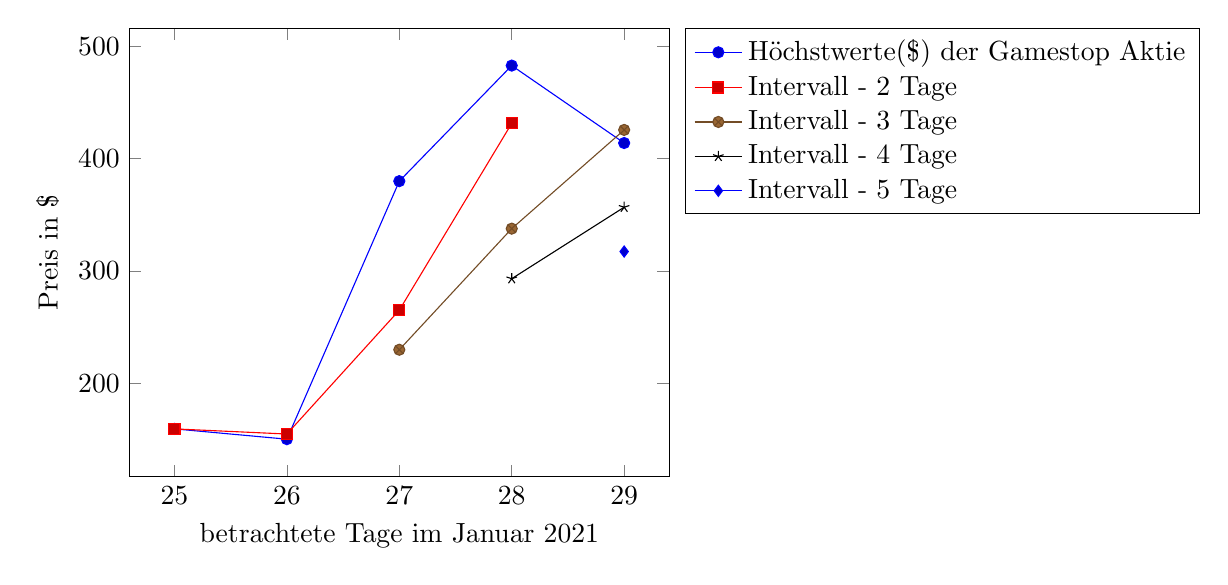
\begin{tikzpicture}
    \begin{axis}[
    xlabel=betrachtete Tage im Januar 2021,
    ylabel=Preis in \$,
    legend pos={outer north east},
    legend cell align={left}
]
        \addplot coordinates {
        	(25, 159.18)
        	(26, 150)
        	(27, 380)
        	(28, 483)
        	(29, 413.98)
        };
        
        \addplot coordinates {
        (25, 159.18)
        (26, 154.59)
        (27, 265)
        (28, 431.5)
        };
        \addplot coordinates {
        (27,229.7266667)
        (28,337.6666667)
        (29,425.66)
        };
        
        \addplot coordinates {
        (28,	293.045)
        (29,	356.745)
        };
        
        \addplot coordinates {
        (29,	317.232)
        };
        \legend{Höchstwerte(\$) der Gamestop Aktie,Intervall - 2 Tage,Intervall - 3 Tage,Intervall - 4 Tage,Intervall - 5 Tage};
    \end{axis}
\end{tikzpicture}
\caption{Gleitender Durchschnitt des Tageshöchstwertes eines Aktienkurses}
\label{abb:gleitendeDurchschnitte}
\end{figure}

% $M_t = (\sum_{T=1}^{t-1}  x_T + x_t )\cdot \frac{1}{T + t}$





\subsection{Bestehende Referenzarchitekturkategorien}
Im Bereich der Streamingarchitekturen gibt es bereits etabblierte Referenzarchitekturen, welche verschiedene mögliche Aufbauarten einer Verarbeitung von Streaming/Zeitreihendaten zeigen.

\begin{figure}[H]
\centering
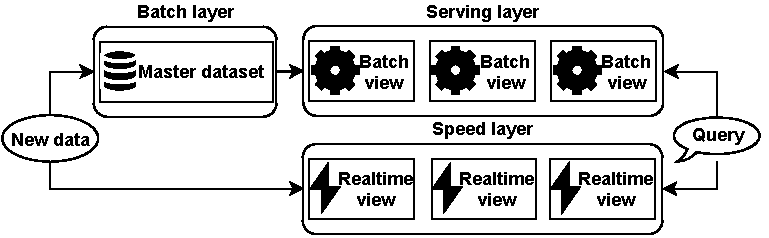
\includegraphics[width=\textwidth]{graphics/Lambda-Reference-Architecture.pdf}
\caption[Die $\lambda$-Datenstreaming Referenzarchitetktur]{Die $\lambda$-Datenstreaming Referenzarchitetktur.\footnotemark}
\label{abb:LambdaStreaming}
\end{figure}
\footnotetext{Mit Änderungen entnommen aus: \cite[][28]{Marz.2015}}
% Lambda nach \citeauthor{Marz.2015}, siehe \footcite[Vgl.][28]{Marz.2015}

Die von \citeauthor{Marz.2015} vorgestellte $\lambda$/Lambda-Architektur, welche in \autoref{abb:LambdaStreaming} gezeigt wird, ist dabei eine der sehr bekannten Referenzarchitekturen. 
Der Name ist dabei nicht mit dem \ac{AWS} Dienst Lambda zu verwechseln, sondern ist wohl auf den gedrehten Buchstaben $\lambda$ zurückzuführen, also \reflectbox{\rotatebox[origin=c]{270}{$\lambda$}}.\footcite[Vgl. auch im Folgenden][]{Berle.27.11.2017} Die $\lambda$-Architektur sieht ausgehend von den hereingeladenen Daten zwei verschiedene Wege für die Daten vor. 
Zum einen den \enquote{Speed Layer}, welcher Daten direkt nach Eingang verarbeitet und nicht im Layer selbst speichert, sondern nur Aggregate oder Ergebnisse zur Verfügung stellt. Zum anderen gibt es den \enquote{Batch layer}, in welchem Daten zuerst in einem Master dataset gespeichert werden und dann in einem festen Intervall (\enquote{Batch jobs}) ausgewertet werden. 
Verschiedene Datenverarbeitungsintervalle machen speziell im Sinne der verschiedenen, in \autoref{abb:DataHalflife} gezeigten, Datenhalbwertszeiten Sinn. So sind manche Auswertungen, die präzise historische Daten benötigen, in einem Batch layer besser möglich als in einem speed layer. Der speed layer bietet dagegen durch die Geschwindigkeit der Auswertungen die Möglichkeit, agil auf erkannte Ereignisse oder Veränderungen im Generellen zu reagieren.


\begin{figure}[H]
\centering
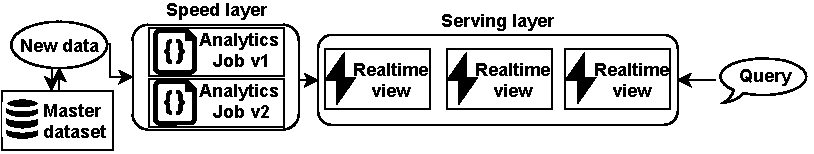
\includegraphics[width=\textwidth]{graphics/Kappa-Reference-Architecture.pdf}
\caption[Die $\kappa$-Datenstreaming Referenzarchitetktur]{Die $\kappa$-Datenstreaming Referenzarchitektur.\footnotemark}
\label{abb:KappaStreaming}
\end{figure}
\footnotetext{Mit Änderungen entnommen aus: \cite{Kreps.2014}, \cite{Berle.27.11.2017}}

Die $\kappa$/Kappa Referenzarchitektur von \citeauthor{Kreps.2014}, dargestellt in \autoref{abb:KappaStreaming} basiert auf der $\lambda$-Architektur, spart jedoch den \enquote{Batch layer} mit zugehörigen \enquote{Batch jobs} aus. 
Das Konzept von Master Data existiert dabei weiterhin, jedoch in Form von Nachrichten, die in einem Messagebroker gespeichert werden. Analysen werden in Form von einzeln versionierten Jobs über die vorhandenen Werte erstellt. 
Wird die Analyse in irgendeiner Weise verändert (z.B. durch Codeanpassungen) werden alle zwischengespeicherten Nachrichten erneut durch eine neue, unveränderliche Version des Jobs analysiert. Diese Unveränderlichkeit hat den Vorteil, dass keine unerwünschten Seiteneffekte durch Analysen, die gegenseitig Ergebnisse überschreiben auftreten. 

% Kappa nach \citeauthor{Kreps.2014},
% siehe \footcite[Vgl.][]{Kreps.2014}



\begin{figure}[H]
\centering
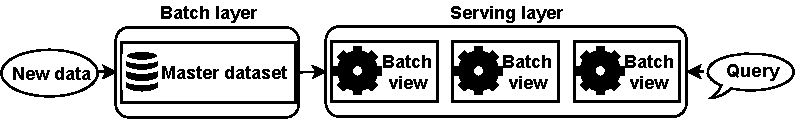
\includegraphics[width=\textwidth]{graphics/OLAP-Reference-Architecture.pdf}
\caption[OLAP Referenzarchitetktur]{OLAP Referenzarchitetktur.\footnotemark}
\label{abb:OLAPStreaming}
\end{figure}
\footnotetext{Mit Änderungen entnommen aus: \cite{Kreps.2014}}

%\ac{OLAP}
Aus der $\lambda$ Referenzarchitektur lässt sich auch eine, zur $\kappa$ Architektur gegenteilige Architektur aufzeigen, welche ein klassisches \ac{OLAP} Szenario aufzeigt. \Todo{Codd zitieren} Diese Architektur basiert, wie in \autoref{abb:OLAPStreaming} gezeigt, auf einer periodischen Verarbeitung der Daten im Master dataset. Dieses Vorgehen ist bei traditionellen Analytics weit verbreitet, bietet jedoch womöglich wichtige Einsichten erst, nachdem die Datenhalbwertszeit bereits überschritten wurde.

% \Todo{Grafik Data Analytics Pipeline}
% \begin{figure}[H]
% \centering
% 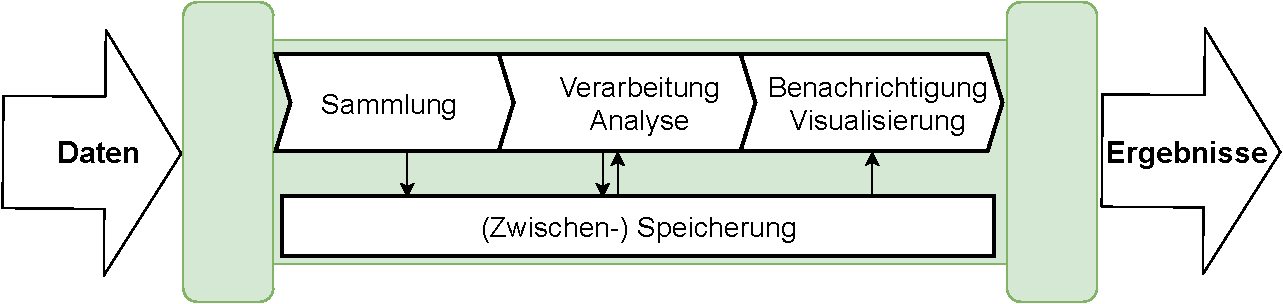
\includegraphics[width=\textwidth]{graphics/DataPipeline.pdf}
% \caption[Aufbau und Ablauf in einer Data Pipeline]{Aufbau und Ablauf in einer Data Pipeline.\footnotemark}
% \label{abb:DataPipeline}
% \end{figure}
% \footnotetext{Mit Änderungen entnommen aus: \cite[][]{}}
% \Todo{Quellenangabe}



\subsection{Echtzeitverarbeitung}
Gemäß der in \autoref{abb:KappaStreaming} gezeigten $\kappa$-Architektur gibt es Nutzungsfälle, in welchen eine reine Echtzeitauswertung basierend auf einer Datenquelle, wie beispielsweise dem Messagebroker, Sinn machen kann. \citeauthor{Belur.2020} sieht dabei vier verschiedene Verwendungszwecke, in welchen die niedrige Verarbeitungslatenz besonders wichtig ist und den maximalen Wert aus den Daten zieht.\footcite[Vgl. auch im Folgenden][]{Belur.2020} Durch Echtzeitreporting und die Erstellung von Dashboards können aktuelle Daten schnell übersichtlich aufbereitet werden. Mittels erstellter Regeln, die Schwellwertüberschreitungen und Anomalien detektieren, können Nutzende benachrichtigt werden, sobald es zu einer Abweichung kommt. Ebenfalls sinnvoll ist der Einsatz von Machine Learning zum Auffinden von Mustern in Daten, was verbesserte Anomalierkennung, Vorraussagen und ähnliche Features ermöglicht. Ein weiterer valider Usecase der $\kappa$-Architektur ist die Transformation von Daten in gewisse Zielformate, um beispielsweise Drittsysteme anzusprechen.




\subsection{Batch Verarbeitung}

Gemäß der in \autoref{abb:OLAPStreaming} gezeigten \ac{OLAP} Architektur, gibt es, wie für die Echtzeitverarbeitung auch nutzende Unternehmen, die ein Entscheidungstempo mit weiterem Horizont haben. Für diese Entscheidungstypen ist dabei wichtig, dass eine Analyse möglichst viele historische Daten umfasst. Es ist dabei aber nicht so wichtig, wie zeitnah diese erstellt werden kann. 
Eine gängige Möglichkeit um effizient alte Daten zu analysieren, stellen \ac{OLAP} Datenbanken dar, welche durch spezielle Indexstrukturen und Optimierungen auf komplexe lesende Abfragen bei großen Datenmengen optimiert wurden. \Todo{belegen} Mittels dieser \ac{OLAP} Datenbanken lassen sich dank der jeweiligen Abfragesprachen und -dialekte komplizierte Abfragen realisieren. Bekanntes Beispiel für so eine Abfragesprache wäre \ac{SQL}, welches einige verschiedene Implementierungen (Dialekte) hat, die verwendet werden können. 